\section{Teorema de Sharkovsky}

%--------------------

\begin{frame}
\vspace{5pt}
\frametitle{Teorema de Sharkovsky}
\begin{columns}
\column{\dimexpr\paperwidth-15pt}

Nessa seção, vamos considerar $f: \RR \to \RR$ uma função contínua.
Além disso, escreveremos $I_0 \longrightarrow I_1 \longrightarrow \cdots \longrightarrow I_n$ quando $I_0, \, I_1, \, \dots, \, I_n$ são intervalos compactos e $f(I_k) \supset I_{k+1}$ para todo $0 \leq k < n$.

\end{columns}
\end{frame}

%--------------------

\begin{frame}
\vspace{5pt}
\frametitle{Teorema de Sharkovsky}
\begin{columns}
\column{\dimexpr\paperwidth-15pt}

\begin{proposition}
Se $I_0 \longrightarrow I_1$, então existe um intervalo fechado $I_0' \subset I_0$ tal que $f(I_0') = I_1$.
\end{proposition}

\begin{proof}
Se $I_0 = [a, b]$ e $I_1 = [c, d]$, sejam $p, \, q \in [a, b]$ tais que $f(p) = c$ e $f(q) = d$.
Suponha que $p \leq q$; se $q \leq p$, a demostração é análoga.

Definindo $b' = \inf \lbrace x \in [p, q] : f(x) = d \rbrace$ e $a' = \sup \lbrace x \in [p, b'] : f(x) = c \rbrace$ e observando que $f$ é contínua, podemos concluir que $f(I_0') = I_1$, onde $I_0' = [a', b']$.
\end{proof}

\end{columns}
\end{frame}

%--------------------

\begin{frame}
\vspace{5pt}
\frametitle{Teorema de Sharkovsky}
\begin{columns}
\column{\dimexpr\paperwidth-15pt}

\begin{lemma}
Se $I_0 \longrightarrow I_1 \longrightarrow \cdots \longrightarrow I_{n-1} \longrightarrow I_0$, então existe $p \in I_0$ tal que as seguintes condições são válidas:
\begin{enumerate}
\item $f^k(p) \in I_k$ para todo $1 \leq k < n$.
\item $f^n(p) = p$.
\end{enumerate}
\end{lemma}

\begin{proof}
Basta observar que podemos construir uma sequência de intervalos fechados $I_0', \, I_1', \, \dots, \, I_{n-1}'$ com as seguintes propriedades:
\begin{enumerate}[a)]
\item \textit{$I_0 \supset I_0' \supset I_1' \supset \cdots \supset I_{n-1}'$.}
\item \textit{$f^k(I_{k-1}') = I_k$ para todo $1 \leq k < n$.}
\item \textit{$f^n(I_{n-1}') = I_0$.}
\qedhere
\end{enumerate}

\end{proof}

\end{columns}
\end{frame}

%--------------------

\begin{frame}
\vspace{5pt}
\frametitle{Teorema de Sharkovsky}
\begin{columns}
\column{\dimexpr\paperwidth-15pt}

\begin{theorem}\label{teo 9-2}
Se $\per_3(f) \neq \emptyset$, então $\per_n(f) \neq \emptyset$ para todo $n \geq 1$.
\end{theorem}

\begin{block}{Demonstração.}
Sejam $p_1 < p_2 < p_3$ os pontos da órbita de um elemento de $\per_3(f)$. Suponha que $f(p_1) = p_2$ e $f(p_2) = p_3$; se $f(p_1) = p_3$ e $f(p_3) = p_2$, a demonstração é análoga.
Definindo $I_0 = [p_1, p_2]$ e $I_1 = [p_2, p_3]$, temos que $I_0 \longrightarrow I_1$, $I_1 \longrightarrow I_0$ e $I_1 \longrightarrow I_1$. Desse modo, podemos demonstrar as seguintes afirmações:

\begin{enumerate}[a)]
\item \textit{$\per_1(f) \neq \emptyset$.}

De fato, $I_1 \longrightarrow I_1$ implica que existe $p \in I_1$ tal que $f(p) = p$.

\item \textit{$\per_2(f) \neq \emptyset$.}

De fato, $I_0 \longrightarrow I_1 \longrightarrow I_0$ implica que existe $p \in I_0$ tal que $f(p) \in I_1$ e $f^2(p) = p$.
Se $f(p) = p$, então $p \in I_0 \cap I_1$, o que é um absurdo pois $I_0 \cap I_1 = \lbrace p_2 \rbrace$ e $p_2 \in \per_3(f)$.
\end{enumerate}
\end{block}

\end{columns}
\end{frame}

%--------------------

\begin{frame}
\vspace{5pt}
\frametitle{Teorema de Sharkovsky}
\begin{columns}
\column{\dimexpr\paperwidth-15pt}

\begin{block}{Demonstração (continuação).}
\begin{enumerate}
\item[c)] \textit{$\per_4(f) \neq \emptyset$.}

De fato, $I_1 \longrightarrow I_1 \longrightarrow I_1 \longrightarrow I_0 \longrightarrow I_1$ implica que existe $p \in I_1$ tal que $f^k(p) \in I_1$ para todo $1 \leq k < 3$, $f^3(p) \in I_0$ e $f^4(p) = p$.

Se $f^3(p) = p$, então $p \in I_0 \cap I_1$, o que é um absurdo pois $I_0 \cap I_1 = \lbrace p_2 \rbrace$ e $f^2(p_2) = p_1 \notin I_1$.
Se $f^k(p) = p$ para algum $1 \leq k < 3$, então $f^k(p) \in I_1$ para todo $k \geq 1$.
Em particular, $f^3(p) \in I_0 \cap I_1 = \lbrace p_2 \rbrace$ e, portanto, $f^4(p) = p = p_3$, o que é um absurdo pois $f(p_3) = p_1 \notin I_1$.
\end{enumerate}
De maneira análoga, podemos mostrar que $\per_n(f) \neq \emptyset$ para todo $n \geq 5$.
\qed
\end{block}

\end{columns}
\end{frame}

%--------------------

\begin{frame}
\vspace{5pt}
\frametitle{Teorema de Sharkovsky}
\begin{columns}
\column{\dimexpr\paperwidth-15pt}

\begin{definition}[Ordenação de Sharkovsky]
$3 \, \triangleright \, 5 
\, \triangleright \, \cdots \, \triangleright \,
2 \cdot 3 \, \triangleright \, 2 \cdot 5 
\, \triangleright \, \cdots \, \triangleright \,
2^2 \cdot 3 \, \triangleright \, 2^2 \cdot 5
\, \triangleright \, \cdots \, \triangleright \,
2^k \cdot 3 \, \triangleright \, 2^k \cdot 5
\, \triangleright \, \cdots \, \triangleright \,
2^2 \, \triangleright \, 2 \, \triangleright \, 1$
\end{definition}
\vspace{15pt}
\begin{theorem}[Sharkovsky]
Se $\per_n(f) \neq \emptyset$, então $\per_m(f) \neq \emptyset$ para todo $n \, \triangleright \, m$.
\end{theorem}

\begin{proof}
Ver \cite{burns}.
\end{proof}

\end{columns}
\end{frame}

%--------------------

\begin{frame}
\vspace{5pt}
\frametitle{Teorema de Sharkovsky}
\begin{columns}
\column{\dimexpr\paperwidth-15pt}

O Teorema de Sharkovsky pode ser usado para provar que órbitas periódicas de certos tamanhos não existem. Por exemplo, observando os gráficos de $h$, $h^2$ e $h^4$ para $\mu = 3.2$ vemos que $\per_4(h) = \emptyset$ e, portanto, $\per_n(h) = \emptyset$ para todo $n \geq 3$.

\begin{figure}[!htb]
\centering
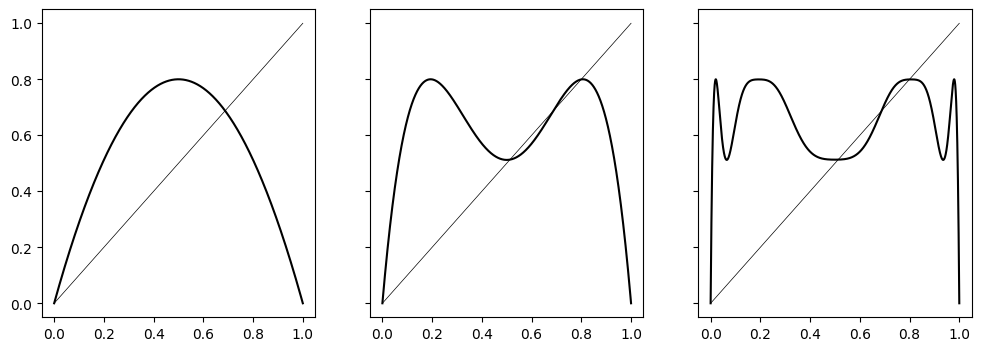
\includegraphics[scale=0.4]{images/h_3,2.png}
\caption{Gráficos de $h$, $h^2$ e $h^4$ para $\mu = 3.2$.}
\label{h_3,2}
\end{figure}

\end{columns}
\end{frame}

%--------------------

\begin{frame}
\vspace{5pt}
\frametitle{Teorema de Sharkovsky}
\begin{columns}
\column{\dimexpr\paperwidth-15pt}

A ordenação de Sharkovsky é a melhor possível. Por exemplo, se $\per_5(f) \neq \emptyset$ implica que $\per_3(f) \neq \emptyset$, então os números $3$ e $5$ podem trocar de lugar nessa ordenação. O seguinte teorema mostra que isso não é possível.

\begin{theorem}
Se $n \geq 1$, então existe uma função $f$ com as seguintes propriedades:
\begin{enumerate}
\item $\per_n(f) \neq \emptyset$.
\item $\per_m(f) =  \emptyset$ para todo $m \, \triangleright \, n$.
\end{enumerate}
\end{theorem}

\end{columns}
\end{frame}
